% ============================================================
%  SmartSupply — Informe de Tesis
%  Estructura basada en Tabarroni_S_Desarrollo_de_Sistema_de_Predicciones_2025.pdf
%  Facultad de Ingeniería — Ingeniería Civil Informática — UNAB
% ============================================================

\documentclass[12pt, a4paper]{report}

% ── Paquetes ─────────────────────────────────────────────────
\usepackage[utf8]{inputenc}
\usepackage[T1]{fontenc}
\usepackage[spanish,es-nodecimaldot]{babel}
\AtBeginDocument{%
  \renewcommand{\contentsname}{Índice de Contenidos}
  \renewcommand{\listfigurename}{Índice de Figuras}
  \renewcommand{\listtablename}{Índice de Tablas}
  \renewcommand{\tablename}{Tabla}
  \renewcommand{\figurename}{Figura}
}
\usepackage{geometry}
\usepackage{graphicx}
\usepackage{hyperref}
\usepackage{booktabs}
\usepackage{longtable}
\usepackage{array}
\usepackage{xcolor}
\usepackage{setspace}
\usepackage{titlesec}
\usepackage{fancyhdr}
\usepackage{caption}
\usepackage{subcaption}
\usepackage{amsmath}
\usepackage{float}
\usepackage{enumitem}
\usepackage{parskip}
\usepackage{lmodern}

% ── Márgenes ─────────────────────────────────────────────────
\geometry{
  top    = 2.5cm,
  bottom = 2.5cm,
  left   = 3cm,
  right  = 2.5cm,
  headheight = 15pt
}

% ── Interlineado ─────────────────────────────────────────────
\onehalfspacing
\setlength{\emergencystretch}{3em}  % evita desbordes con identificadores largos en \texttt

% ── Colores UNAB ─────────────────────────────────────────────
\definecolor{unabblue}{RGB}{31,56,100}
\definecolor{unablight}{RGB}{46,117,182}

% ── Estilo de títulos ─────────────────────────────────────────
\titleformat{\chapter}[block]
  {\normalfont\Large\bfseries\color{unabblue}}
  {\thechapter.}{1em}{}
\titleformat{\section}[block]
  {\normalfont\large\bfseries\color{unablight}}
  {\thesection.}{0.8em}{}
\titleformat{\subsection}[block]
  {\normalfont\normalsize\bfseries}
  {\thesubsection.}{0.6em}{}
\titleformat{\subsubsection}[block]
  {\normalfont\normalsize\itshape}
  {\thesubsubsection.}{0.5em}{}

% ── Encabezado / pie de página ────────────────────────────────
\pagestyle{fancy}
\fancyhf{}
\fancyhead[L]{\small\textit{SmartSupply — Predicción de Demanda y Reabastecimiento}}
\fancyhead[R]{\small\thepage}
\renewcommand{\headrulewidth}{0.4pt}

% ── Hipervínculos ─────────────────────────────────────────────
\hypersetup{
  colorlinks = true,
  linkcolor  = unabblue,
  citecolor  = unabblue,
  urlcolor   = unablight
}

% ============================================================
\begin{document}

% ── Portada ──────────────────────────────────────────────────
\begin{titlepage}
  \centering
  \vspace*{1cm}

  % Logo UNAB: descargar desde repositorio.unab.cl y guardar como figuras/logo_unab.png
  
\includegraphics[width=0.30\textwidth]{figuras/logo_unab.png}\\[0.4cm]

  {\Large \textbf{Facultad de Ingeniería}}\\[0.2cm]
  {\large Ingeniería Civil Informática}

  \vfill

  {\LARGE \textbf{\color{unabblue}
    PLATAFORMA DE PREDICCIÓN DE DEMANDA Y\\[0.3cm]
    REABASTECIMIENTO AUTOMÁTICO PARA\\[0.3cm]
    EMPRENDIMIENTOS Y NEGOCIOS EN CRECIMIENTO\\[0.3cm]
    MEDIANTE SELECCIÓN AUTOMÁTICA DE MODELOS (AMS)
  }}\\[1cm]

  

  \vfill

  \textbf{Autores:}\\[0.2cm]
  Matias Muñoz Parraguirre\\
  Ignacio Duarte Miranda\\
  Cristóbal Flores Villegas\\[0.8cm]

  \textbf{Profesor guía:}\\[0.2cm]
  Paulo Luis Francisco Quinsacara Jofré

  \vfill

  Santiago, Chile\\[0.1cm]
  \today
\end{titlepage}


% ── Índices ──────────────────────────────────────────────────
\tableofcontents
\newpage
\listoffigures
\newpage
\listoftables
\newpage

% ── Resumen ──────────────────────────────────────────────────
\chapter*{Resumen}
\addcontentsline{toc}{chapter}{Resumen}

La gestión del inventario y la predicción de demanda representan uno de los mayores
desafíos operacionales para emprendimientos y negocios en crecimiento. Las soluciones
existentes —como SAP o Oracle— son costosas y requieren implementaciones largas,
quedando fuera del alcance de la mayoría de las pequeñas y medianas empresas. A su vez,
la diversidad de comportamientos de demanda entre productos dificulta la aplicación de un
único modelo de predicción para todos los SKUs.

El presente proyecto propone \textbf{SmartSupply}, una plataforma SaaS de predicción de
demanda y reabastecimiento automático que implementa un mecanismo de Selección
Automática de Modelos (AMS) por SKU, evaluando cuatro algoritmos —ARIMA, Prophet,
XGBoost y LSTM— y seleccionando aquel con menor error de predicción (WAPE) para
cada familia de productos. La hipótesis central plantea que esta selección automática
reduce el error de predicción y el capital inmovilizado frente al uso de un modelo único.

La plataforma integra un pipeline ETL sobre el dataset público \textit{Store Sales — Corporación
Favorita} (Kaggle, 2017) para benchmarking, una API REST construida con FastAPI, un módulo
de gestión de inventario basado en las políticas EOQ y $(s,S)$, y un dashboard web en React.
El sistema incorpora un \textbf{módulo de ingesta inteligente} que utiliza el modelo Claude
(Anthropic) con capacidades de visión para extraer y normalizar datos de ventas desde
imágenes, planillas Excel o PDFs, eliminando la barrera de entrada para negocios sin
sistemas digitalizados. La arquitectura es \textbf{multi-tenant} y escalable: cada negocio
opera de forma aislada sobre la misma infraestructura mediante \texttt{business\_id}.

Los resultados obtenidos sobre datos reales muestran que el AMS selecciona el modelo
óptimo por SKU de forma consistente, con errores WAPE por debajo del 15\,\% en series con
patrones regulares. La metodología de desarrollo sigue el framework ágil Scrum en 5
sprints y el proceso CRISP-DM para el tratamiento de datos.

\textbf{Palabras clave:} predicción de demanda, selección automática de modelos, WAPE,
inventario, EOQ, política $(s,S)$, ARIMA, Prophet, XGBoost, LSTM, FastAPI, React,
ingesta IA, multi-tenancy, emprendimientos, SaaS.

\newpage

% ── Abstract ─────────────────────────────────────────────────
\chapter*{Abstract}
\addcontentsline{toc}{chapter}{Abstract}

Inventory management and demand forecasting represent one of the greatest operational
challenges for startups and growing businesses. Existing enterprise solutions —such as SAP
or Oracle— are cost-prohibitive and require lengthy implementations, placing them out of
reach for most small and medium-sized enterprises. Furthermore, the diversity of demand
behaviors across product families makes it difficult to apply a single forecasting model
to all SKUs.

This project proposes \textbf{SmartSupply}, a SaaS platform for demand forecasting and
automatic restocking that implements an Automatic Model Selection (AMS) mechanism per
SKU, evaluating four algorithms —ARIMA, Prophet, XGBoost and LSTM— and selecting the
one with the lowest forecasting error (WAPE) for each product family. The central
hypothesis is that this per-SKU automatic selection reduces forecasting error and
tied-up capital compared to using a single model for all products.

The platform integrates an ETL pipeline over the public dataset \textit{Store Sales —
Corporación Favorita} (Kaggle, 2017) for benchmarking, a REST API built with FastAPI, an
inventory management module based on EOQ and $(s,S)$ policies, and a React web
dashboard. The system incorporates an \textbf{intelligent ingestion module} that uses the
Claude language model (Anthropic) with vision capabilities to extract and normalize sales
data from images, Excel files or PDFs, eliminating the digital barrier for businesses
without ERP systems. The architecture is \textbf{multi-tenant} and scalable: each
business operates in isolation on the same infrastructure through a unique
\texttt{business\_id}.

Results obtained on real ingested data show that the AMS consistently selects the
optimal model per SKU, achieving WAPE values below 15\,\% on series with regular
patterns. The development methodology follows the Scrum agile framework across 5 sprints
and the CRISP-DM process for data treatment.

\textbf{Keywords:} demand forecasting, automatic model selection, WAPE, inventory, EOQ,
$(s,S)$ policy, ARIMA, Prophet, XGBoost, LSTM, FastAPI, React, AI ingestion,
multi-tenancy, startups, SaaS.

\newpage

% ============================================================
%  CAPÍTULO 1 — INTRODUCCIÓN
% ============================================================
\chapter{Introducción}

\section{Contexto}

En el ecosistema actual de emprendimientos y pequeñas y medianas empresas (PyMEs),
la gestión eficiente del inventario y la predicción de demanda representan desafíos
operacionales críticos. Un quiebre de stock implica ventas perdidas y deterioro de la
relación con el cliente, mientras que un exceso de inventario inmoviliza capital de trabajo
que un emprendimiento en crecimiento no puede permitirse desperdiciar. Ambos escenarios
son consecuencia directa de predicciones de demanda imprecisas o metodologías de
reabastecimiento estáticas.

Las herramientas empresariales existentes para abordar este problema —como SAP,
Oracle NetSuite o Microsoft Dynamics— presentan barreras de entrada significativas en
términos de costo, tiempo de implementación y complejidad técnica, quedando fuera del
alcance de la mayoría de los emprendimientos y negocios en etapa de crecimiento
(Ramírez \& Concha, 2021). Esto genera una brecha tecnológica: mientras las grandes
corporaciones optimizan su inventario con algoritmos avanzados, las empresas más
pequeñas siguen tomando decisiones de compra de forma intuitiva o con hojas de cálculo.

Adicionalmente, muchos emprendimientos no cuentan con datos de ventas en formato
digital estructurado. Sus registros históricos existen en cuadernos, planillas Excel
desordenadas o comprobantes físicos, lo que impide aplicar cualquier modelo predictivo
sin un proceso previo de digitalización y normalización de datos.

La proliferación de algoritmos de \textit{machine learning} y series de tiempo ofrece hoy
múltiples alternativas para el pronóstico de ventas, pero la elección del modelo óptimo
varía según las características de cada producto (estacionalidad, tendencia, presencia de
ceros) y el horizonte de predicción requerido. No existe un único modelo que funcione
bien para todos los SKUs de un mismo negocio.

\section{Planteamiento del Problema}

Los emprendimientos y negocios en crecimiento carecen de herramientas accesibles que
les permitan: (1) digitalizar su historial de ventas desde cualquier formato, (2) predecir
la demanda futura con el modelo estadístico más adecuado para cada producto, y (3)
generar automáticamente políticas de reabastecimiento basadas en esas predicciones.

La pregunta de investigación que guía este proyecto es:

\begin{quote}
\textit{¿En qué medida la selección automática del mejor modelo de forecasting por SKU
reduce el error de predicción y el capital inmovilizado frente al uso de un modelo único
para todos los productos en emprendimientos y negocios en crecimiento?}
\end{quote}

\section{Hipótesis}

La selección automática del mejor modelo de forecasting por SKU (AMS) mediante
validación \textit{walk-forward} reduce el error de predicción global (WAPE) y, en
consecuencia, el capital inmovilizado en inventario, en comparación con el uso de un
modelo único aplicado a todos los productos de un mismo negocio, independientemente
del rubro o tamaño de la empresa.

\section{Importancia del Proyecto}

La selección inadecuada del modelo de forecasting es una de las causas más frecuentes
de error en los sistemas de reabastecimiento. Un modelo que funciona bien para productos
de alta rotación con estacionalidad semanal puede ser completamente inadecuado para
artículos con demanda esporádica o con tendencias de largo plazo. Automatizar esta
selección por SKU, de forma transparente y sin requerir conocimiento técnico por parte
del usuario, permite:

\begin{itemize}
  \item Reducir el error de predicción global (WAPE) respecto al uso de un modelo único.
  \item Disminuir el capital inmovilizado en inventario al calibrar mejor los puntos de
        reorden.
  \item Generar órdenes de compra oportunas y calibradas a la demanda real de cada
        producto.
  \item Eliminar la barrera de digitalización de datos mediante ingesta IA.
  \item Entregar a emprendedores y gestores una herramienta visual accesible, sin
        necesidad de conocimiento en ciencia de datos o sistemas ERP.
  \item Escalar desde un emprendimiento unipersonal hasta una cadena con múltiples
        sucursales, gracias a la arquitectura multi-tenant.
\end{itemize}

\section{Contribución del Proyecto}

SmartSupply realiza los siguientes aportes:

\begin{enumerate}
  \item Un \textbf{módulo AMS} que selecciona automáticamente el mejor modelo de
        forecasting por SKU mediante validación walk-forward (70\,/\,15\,/\,15),
        evaluando ARIMA, Prophet, XGBoost y LSTM.
  \item Un \textbf{módulo de inventario} que aplica EOQ y política $(s,S)$ sobre los
        pronósticos generados por AMS, calculando puntos de reorden y cantidades óptimas
        de pedido.
  \item Una \textbf{API REST} (FastAPI) documentada automáticamente via OpenAPI/Swagger,
        consumible por cualquier sistema externo.
  \item Un \textbf{dashboard web} (React + Recharts) para visualización de pronósticos,
        alertas de inventario, órdenes de compra y KPIs operacionales en tiempo real.
  \item Un \textbf{pipeline ETL} reproducible sobre el dataset Store Sales — Corporación
        Favorita (Kaggle, 2017) para benchmarking y validación de la hipótesis.
  \item Un \textbf{módulo de ingesta inteligente} que utiliza Claude (Anthropic) con
        capacidades de visión y procesamiento de documentos para extraer y normalizar
        datos de ventas desde imágenes, planillas Excel y PDFs, eliminando la barrera
        de entrada para negocios sin sistemas digitalizados.
  \item Una \textbf{arquitectura multi-tenant escalable} que aísla los datos de cada
        negocio mediante \texttt{business\_id}, habilitando el despliegue como plataforma
        SaaS accesible desde un emprendimiento hasta una empresa con múltiples sucursales.
\end{enumerate}

\section{Objetivos}

\subsection{Objetivo General}

Desarrollar una plataforma SaaS de predicción de demanda y reabastecimiento automático
para emprendimientos y negocios en crecimiento que, mediante la selección automática del
mejor modelo de forecasting por SKU, reduzca el error de predicción y el capital
inmovilizado respecto al uso de un modelo único para todos los productos.

\subsection{Objetivos Específicos}

\begin{enumerate}
  \item Implementar y evaluar cuatro modelos de predicción de series de tiempo (ARIMA,
        Prophet, XGBoost y LSTM) sobre el dataset Store Sales — Corporación Favorita,
        como conjunto de benchmarking representativo de negocios con múltiples SKUs.
  \item Desarrollar el mecanismo AMS que selecciona el modelo de menor WAPE por SKU
        mediante validación cruzada temporal (walk-forward con partición 70/15/15).
  \item Implementar las políticas de gestión de inventario EOQ y $(s,S)$ alimentadas
        por los pronósticos del AMS, generando parámetros de reorden por SKU.
  \item Construir una API REST con FastAPI que exponga los módulos de forecasting e
        inventario, con autenticación JWT y arquitectura multi-tenant por
        \texttt{business\_id}.
  \item Desarrollar un dashboard web interactivo en React para la visualización de
        pronósticos, métricas de inventario, gestión de órdenes de compra y KPIs
        operacionales del negocio.
  \item Diseñar e implementar un pipeline ETL que cargue, limpie y normalice el dataset
        de benchmarking en una base de datos PostgreSQL alojada en Supabase.
  \item Desarrollar un módulo de ingesta inteligente basado en IA (Claude, Anthropic) que
        permita a cualquier negocio incorporar sus datos históricos de ventas desde
        cualquier formato digital (imágenes, Excel, PDF), con validación de calidad
        previa a la carga.
\end{enumerate}

\section{Limitaciones del Proyecto}

\begin{itemize}
  \item La validación cuantitativa de la hipótesis se realiza sobre el dataset Store Sales
        — Corporación Favorita (Ecuador, 2013--2017), que actúa como negocio de
        demostración. El módulo de ingesta IA permite incorporar datos reales de cualquier
        negocio en producción.
  \item El AMS evalúa cuatro modelos de forecasting; existen alternativas (SARIMA,
        N-BEATS, Temporal Fusion Transformer) no contempladas en este alcance pero
        integrables en versiones futuras.
  \item El módulo de inventario asume demanda independiente por SKU; no modela
        restricciones de capacidad de bodega ni descuentos por volumen.
  \item La calidad de la extracción del módulo de ingesta IA depende de la legibilidad
        del documento fuente; imágenes de muy baja resolución pueden producir resultados
        incompletos.
  \item La integración bidireccional con sistemas ERP o WMS externos queda fuera del
        alcance de esta tesis; la API REST está disponible para integraciones futuras.
  \item El sistema ha sido validado principalmente con datos de retail y distribución;
        rubros con demanda muy irregular (servicios bajo pedido, proyectos) pueden
        requerir ajustes en los modelos.
\end{itemize}

% ============================================================
%  CAPÍTULO 2 — MARCO TEÓRICO
% ============================================================
\chapter{Marco Teórico}

\section{Metodologías de Trabajo}

Una metodología de trabajo es un conjunto de técnicas, reglas y procedimientos que
estructuran la forma en que un equipo desarrolla un proyecto. Al adoptar una metodología
bien definida se mejora la eficiencia, la calidad de los entregables y la comunicación
interna del equipo.

\subsection{Metodología Scrum}

Scrum es un framework ágil para el desarrollo iterativo e incremental de productos
complejos (Schwaber \& Sutherland, 2020). Se organiza en ciclos de trabajo llamados
\textit{Sprints} de duración fija —en este proyecto, dos semanas— al final de los cuales se
entrega un incremento potencialmente funcional del sistema. Scrum permite que los
equipos se autogestionen, aprendan de la experiencia y se adapten a los cambios del
entorno, características esenciales en proyectos de software con requerimientos evolutivos.

\subsection{¿Cómo funciona Scrum?}

El proceso Scrum comienza con la definición del \textit{Product Backlog}, lista priorizada de
todas las funcionalidades requeridas. En cada \textit{Sprint Planning} el equipo selecciona
los ítems a desarrollar en el siguiente Sprint, generando el \textit{Sprint Backlog}. Diariamente
se realiza una reunión breve (\textit{Daily Scrum}) para sincronizar el avance. Al final del Sprint
se realiza la \textit{Sprint Review} (demo) y la \textit{Sprint Retrospective} (mejora de proceso).

\begin{figure}[H]
  \centering
  % \includegraphics[width=0.75\textwidth]{figuras/scrum_proceso.png}
  \fbox{\parbox{0.75\textwidth}{\centering[Diagrama del proceso Scrum]}}
  \caption{Proceso Scrum — ciclo de sprints}
  \label{fig:scrum}
\end{figure}

\subsection{Roles de Scrum}

Para aplicar la metodología Scrum se definen tres roles esenciales: el Product Owner,
el Scrum Master y el Equipo de Desarrollo. Cada uno tiene responsabilidades específicas
descritas en The Scrum Guide (Schwaber \& Sutherland, 2020).

\begin{table}[H]
  \centering
  \caption{Roles Scrum — SmartSupply}
  \label{tab:roles_scrum}
  \begin{tabular}{|l|l|l|}
    \hline
    \textbf{Rol} & \textbf{Responsabilidad} & \textbf{Integrante} \\
    \hline
    Product Owner & Priorizar Product Backlog, validar entregables & Paulo Quinsacara Jofré \\
    Scrum Master  & Facilitar ceremonias, remover impedimentos     & Matias Muñoz Parraguirre \\
    Dev Team      & Diseño, implementación, pruebas                & Los 3 integrantes \\
    \hline
  \end{tabular}
\end{table}

\subsection{Fases de una Metodología Scrum}

Las fases principales son: Planificación del Sprint, Ejecución del Sprint (con Daily Scrums),
Sprint Review y Sprint Retrospective. Este ciclo se repite durante los sprints planificados.
En SmartSupply se ejecutaron 5 sprints de desarrollo más un sprint final de QA y despliegue.

\subsection{Arquitectura de Software y Modelo de Vistas 4+1}

El modelo de vistas 4+1 (Kruchten, 1995) describe la arquitectura de un sistema de
software a través de cinco perspectivas complementarias:

\begin{itemize}
  \item \textbf{Vista Lógica}: estructura de clases y componentes del dominio.
  \item \textbf{Vista de Procesos}: comportamiento dinámico del sistema en tiempo de
        ejecución (diagramas de secuencia y actividad).
  \item \textbf{Vista de Desarrollo}: organización del código fuente en módulos,
        paquetes y capas (diagrama de componentes).
  \item \textbf{Vista Física}: infraestructura de despliegue, servidores y redes
        (diagrama de despliegue).
  \item \textbf{Vista de Escenarios (``+1'')}: casos de uso que integran las cuatro
        vistas anteriores desde la perspectiva del usuario.
\end{itemize}

SmartSupply aplica este modelo en el Capítulo 5, documentando cada vista con los
diagramas UML correspondientes.

\subsection{Lenguaje de Modelado Gráfico (UML)}

UML (\textit{Unified Modeling Language}) es un estándar de la industria para la
visualización, especificación y documentación de sistemas de software orientados a
objetos (Booch, Rumbaugh \& Jacobson, 1999). En este proyecto se utilizan los
diagramas de clases, secuencia, componentes y despliegue para documentar la
arquitectura del sistema.

\subsection{BPMN}

BPMN (\textit{Business Process Model and Notation}) es un estándar para el modelado
de procesos de negocio mediante una notación gráfica estandarizada (OMG, 2011).
Permite representar flujos de trabajo con participantes, eventos, actividades y
decisiones, facilitando la comunicación entre equipos técnicos y de negocio.
En SmartSupply se utiliza BPMN para modelar el flujo completo del proceso de
ingesta inteligente de datos.

\section{Proceso CRISP-DM}

CRISP-DM (\textit{Cross Industry Standard Process for Data Mining}) es un proceso estándar
para proyectos de ciencia de datos que consta de seis fases (Shearer, 2000):

\begin{enumerate}
  \item \textbf{Business Understanding}: definir el problema de negocio y los criterios
        de éxito. En SmartSupply, esto corresponde a reducir el error de predicción y el
        capital inmovilizado.
  \item \textbf{Data Understanding}: exploración y análisis de calidad de los datos.
        Se analizó el dataset Store Sales — Corporación Favorita y los datos reales
        ingestados por cada negocio.
  \item \textbf{Data Preparation}: limpieza, transformación e ingeniería de
        características. Implementado en \texttt{02\_clean.py} del pipeline ETL.
  \item \textbf{Modeling}: selección y entrenamiento de modelos. Corresponde al módulo
        AMS con los cuatro algoritmos de forecasting.
  \item \textbf{Evaluation}: validación contra métricas de negocio mediante WAPE en
        ventana walk-forward.
  \item \textbf{Deployment}: despliegue del sistema en Render (backend) y Cloudflare
        Pages (frontend).
\end{enumerate}

\section{Modelos de Forecasting}

\subsection{ARIMA}

ARIMA (\textit{Autoregressive Integrated Moving Average}) es un modelo estadístico
clásico para series de tiempo estacionarias (Box \& Jenkins, 1976). Se define por tres
parámetros $(p, d, q)$: orden autorregresivo, grado de diferenciación y orden de media
móvil. En su variante SARIMA se agrega un componente estacional $(P, D, Q)_m$ que
captura ciclos de periodo $m$. En SmartSupply, el AMS realiza una búsqueda en grilla
sobre 144 combinaciones de parámetros, incluyendo componente estacional semanal
($m=7$) cuando la serie cuenta con al menos 21 observaciones.

\subsection{Prophet}

Prophet es un modelo de forecasting desarrollado por Meta (Taylor \& Letham, 2018),
diseñado para manejar estacionalidades múltiples, efectos de feriados y valores
atípicos. Descompone la serie en tendencia, estacionalidad y calendario. En SmartSupply,
la estacionalidad anual se activa dinámicamente solo cuando la serie tiene 730 o más
días de historia, evitando el sobreajuste en series cortas.

\subsection{XGBoost}

XGBoost (\textit{Extreme Gradient Boosting}) es un algoritmo de ensamble basado en
árboles de decisión (Chen \& Guestrin, 2016). Para series de tiempo se aplica mediante
ingeniería de características temporales: lags de ventas, medias móviles, variables de
calendario (día de semana, mes) y features exógenas (feriados). En SmartSupply se
implementa con la estrategia DIRMO (\textit{Direct Multi-Output}), donde se entrena un
modelo independiente por cada horizonte de predicción, evitando la acumulación de
error en predicciones multi-paso.

\subsection{LSTM}

Las redes LSTM (\textit{Long Short-Term Memory}) son una variante de las redes
neuronales recurrentes que resuelven el problema del gradiente desvanecido mediante
compuertas de entrada, olvido y salida (Hochreiter \& Schmidhuber, 1997). Son
especialmente efectivas para capturar dependencias de largo plazo en series temporales.
En SmartSupply, el modelo LSTM está implementado en PyTorch con la estrategia DIRMO
y utiliza seis \textit{features} de entrada: ventas históricas, componentes seno/coseno del
día de semana y del mes, e indicador de feriado chileno. Incluye corrección automática
de días de cierre basada en el historial de demanda cero por día de semana.

\section{Selección Automática de Modelos (AMS)}

El AMS (\textit{Automatic Model Selection}) implementa validación \textit{walk-forward}:
el historial de ventas de cada SKU se divide en 70\,\% entrenamiento, 15\,\% validación
y 15\,\% prueba. Para cada SKU, los cuatro modelos se entrenan y evalúan sobre la
ventana de validación; el de menor WAPE se designa como modelo activo para ese SKU
y genera las predicciones del horizonte solicitado.

Se utiliza el WAPE (\textit{Weighted Absolute Percentage Error}) en lugar del MAPE
clásico, ya que el MAPE es inestable cuando la demanda real $y_t$ se acerca a cero —
condición frecuente en series de ventas con días sin actividad. La fórmula del WAPE es:

\[
  \text{WAPE} = \frac{\displaystyle\sum_{t=1}^{n} |y_t - \hat{y}_t|}
                     {\displaystyle\sum_{t=1}^{n} y_t} \times 100\%
\]

donde $y_t$ es el valor real y $\hat{y}_t$ el valor predicho. Al ponderar el error por
el volumen total de ventas, el WAPE es más robusto ante valores nulos y refleja mejor
el impacto económico del error de predicción.

\section{Gestión de Inventario}

\subsection{Modelo EOQ}

El \textit{Economic Order Quantity} (EOQ) determina la cantidad óptima de pedido que
minimiza los costos totales de inventario, combinando el costo de hacer un pedido y el
costo de mantener unidades en stock (Harris, 1913):

\[
  Q^* = \sqrt{\frac{2 D K}{h}}
\]

donde $D$ es la demanda anual proyectada por el AMS, $K$ el costo fijo por orden de
compra y $h$ el costo de mantención por unidad por año.

\subsection{Política $(s,S)$}

La política de inventario $(s,S)$ establece dos parámetros: el punto de reorden $s$ (nivel
mínimo de stock que dispara un pedido) y el nivel objetivo $S$ (nivel al que se repone
el inventario tras el pedido). Cuando el stock cae por debajo de $s$, se genera una
orden por $Q = S - \text{stock actual}$ unidades (Silver, Pyke \& Peterson, 1998).
Los parámetros se calculan como:

\[
  s = \bar{d} \cdot L + z_\alpha \cdot \sigma_d \cdot \sqrt{L}
  \qquad
  S = s + Q^*
\]

donde $\bar{d}$ es la demanda media diaria del AMS, $L$ el \textit{lead time} en días,
$\sigma_d$ la desviación estándar de la demanda y $z_\alpha$ el factor de servicio.

\section{Herramientas de Desarrollo}

\subsection{Python 3.11}

Python es el lenguaje principal del proyecto, utilizado en el backend, ETL y módulos
de forecasting. Se emplea la versión 3.11 por su compatibilidad con las bibliotecas
de machine learning utilizadas. Las dependencias se gestionan mediante un entorno
virtual (\texttt{venv}).

\subsection{FastAPI}

FastAPI es un framework web moderno para Python que genera automáticamente
documentación OpenAPI/Swagger a partir de las anotaciones de tipo del código
(Ramírez, 2018). Ofrece validación automática de datos mediante Pydantic y rendimiento
comparable a frameworks asíncronos de Node.js.

\subsection{React y Vite}

React es una biblioteca JavaScript para construir interfaces de usuario basadas en
componentes reutilizables (Meta, 2013). Vite actúa como bundler de desarrollo con
recarga en caliente. En SmartSupply el frontend utiliza React 18 con TanStack Query
para gestión de estado del servidor, Recharts para visualizaciones y Zustand para
estado de autenticación.

\subsection{PostgreSQL y Supabase}

PostgreSQL es el sistema de gestión de base de datos relacional del proyecto.
Supabase provee PostgreSQL como servicio gestionado en la nube, incluyendo
autenticación, Row Level Security (RLS) y una API REST automática. SmartSupply
utiliza la capa de conexión directa vía SQLAlchemy 2.0 sobre el \textit{connection pooler}
de Supabase.

\subsection{Claude API (Anthropic)}

Claude es un modelo de lenguaje grande (LLM) desarrollado por Anthropic con
capacidades de visión y procesamiento de documentos. En SmartSupply se utilizan
dos variantes: \texttt{claude-haiku-4-5} para extracción de imágenes y PDFs (menor
latencia) y \texttt{claude-sonnet-4-6} para mapeo de columnas en planillas Excel con
nomenclatura ambigua (mayor razonamiento). La integración se realiza mediante el
SDK oficial de Anthropic para Python.

\subsection{PyTorch}

PyTorch es una biblioteca de aprendizaje profundo de código abierto desarrollada por
Meta AI. En SmartSupply se utiliza para implementar el modelo LSTM, aprovechando
su API dinámica de grafos de cómputo y facilidad de depuración respecto a alternativas
basadas en grafos estáticos.

\subsection{Pandas y Bibliotecas Científicas}

Pandas es la biblioteca central para manipulación de datos tabulares en Python. Se
complementa con \texttt{statsmodels} (ARIMA/SARIMA), \texttt{prophet} (Meta Prophet),
\texttt{xgboost} (algoritmo de ensamble) y \texttt{scikit-learn} (métricas y utilidades
de validación).

\section{Multi-tenancy y Arquitectura SaaS}

Una arquitectura \textit{multi-tenant} permite que múltiples clientes (tenants) compartan
la misma infraestructura de software manteniendo sus datos completamente aislados
(Curino et al., 2010). Este modelo es la base de las plataformas SaaS
(\textit{Software as a Service}), donde el proveedor opera un único sistema y cada cliente
accede a su instancia lógica mediante credenciales y un identificador único.

En SmartSupply, cada negocio registrado recibe un \texttt{business\_id} único. Todas las
tablas de la base de datos (\texttt{sales\_history}, \texttt{products}, \texttt{stock\_levels},
\texttt{purchase\_orders}, \texttt{ingest\_log}) incluyen \texttt{business\_id} como clave
de partición lógica. Los endpoints de la API filtran automáticamente los datos por el
negocio del usuario autenticado, garantizando el aislamiento. Esta arquitectura permite
que SmartSupply escale desde un emprendimiento unipersonal hasta una cadena con
múltiples sucursales sin cambios en la infraestructura.

\section{Dataset: Store Sales — Corporación Favorita}

El dataset público Store Sales — Corporación Favorita (Kaggle, 2017) contiene datos
reales de ventas de 54 tiendas en Ecuador durante el período 2013--2017. Se utiliza en
SmartSupply como conjunto de benchmarking para entrenar y evaluar el AMS sobre un
volumen de datos representativo de un negocio con múltiples SKUs y sucursales. Sus
características se resumen en la Tabla~\ref{tab:dataset}.

\begin{table}[H]
  \centering
  \caption{Características del Dataset Store Sales — Corporación Favorita}
  \label{tab:dataset}
  \begin{tabular}{|l|l|}
    \hline
    \textbf{Característica} & \textbf{Valor} \\
    \hline
    Período          & 2013-01-01 a 2017-08-15 \\
    Filas (train)    & 3.000.888 \\
    Tiendas          & 54 \\
    Familias (SKUs)  & 33 \\
    Columnas         & id, date, store\_nbr, family, sales, onpromotion \\
    Demanda cero     & \textasciitilde 31,3\,\% de los registros \\
    Archivos extra   & stores.csv, oil.csv, holidays\_events.csv, transactions.csv \\
    \hline
  \end{tabular}
\end{table}

% ============================================================
%  CAPÍTULO 3 — IDENTIFICACIÓN DE REQUISITOS
% ============================================================
\chapter{Identificación de Requisitos}

\section{Partes Interesadas (Stakeholders)}

\begin{table}[H]
  \centering
  \caption{Stakeholders de SmartSupply}
  \label{tab:stakeholders}
  \begin{tabular}{|l|l|l|}
    \hline
    \textbf{Stakeholder} & \textbf{Interés} & \textbf{Influencia} \\
    \hline
    Emprendedor / Dueño del negocio & Controlar inventario, reducir capital inmovilizado & Alta \\
    Encargado de Operaciones        & Gestionar órdenes de compra, evitar quiebres de stock & Alta \\
    Analista / Supervisor           & Monitorear métricas de predicción y nivel de servicio & Media \\
    Inversionistas / Dirección      & Reducir costos operacionales y mejorar rentabilidad   & Alta \\
    Equipo de TI (si existe)        & Integración con sistemas existentes vía API REST       & Media \\
    \hline
  \end{tabular}
\end{table}

\section{Usuarios}

Los usuarios directos del sistema son:

\begin{itemize}
  \item \textbf{Administrador} (dueño o fundador del negocio): registra el negocio,
        carga datos históricos de ventas, gestiona productos y parámetros de inventario,
        y tiene acceso completo a todas las funciones del sistema.
  \item \textbf{Operador} (encargado de operaciones o bodega): consulta alertas de
        inventario, genera órdenes de compra, monitorea el estado de los pedidos y
        utiliza el asistente Stocky para consultas en lenguaje natural.
\end{itemize}

\section{Roles}

Los roles del sistema son:

\begin{itemize}
  \item \textbf{Administrador}: acceso completo — gestión de negocios, productos,
        datos, forecasting, inventario e ingesta IA.
  \item \textbf{Analista}: visualización de dashboards, forecasts, alertas y órdenes
        de compra; sin acceso a configuración de parámetros del sistema.
\end{itemize}

\section{Requisitos del Sistema}

A continuación se describen los requisitos funcionales principales del sistema.

\begin{table}[H]
  \centering
  \caption{Requisito RF-01: Autenticación de Usuarios}
  \label{tab:rf01}
  \begin{tabular}{|l|p{9cm}|}
    \hline
    \textbf{Campo} & \textbf{Descripción} \\
    \hline
    ID          & RF-01 \\
    Nombre      & Autenticación de Usuarios \\
    Descripción & El sistema debe permitir el registro e inicio de sesión mediante
                  correo y contraseña, generando un token JWT con expiración configurable.
                  Los endpoints protegidos deben rechazar solicitudes sin token válido. \\
    Actor       & Todos los usuarios \\
    Prioridad   & Alta \\
    \hline
  \end{tabular}
\end{table}

\begin{table}[H]
  \centering
  \caption{Requisito RF-02: Registrar Negocio en el Sistema}
  \label{tab:rf02}
  \begin{tabular}{|l|p{9cm}|}
    \hline
    \textbf{Campo} & \textbf{Descripción} \\
    \hline
    ID          & RF-02 \\
    Nombre      & Registrar Negocio en el Sistema \\
    Descripción & El sistema debe permitir registrar un emprendimiento o negocio con
                  nombre, RUT y ciudad, asignándole un \texttt{business\_id} único que
                  aísla sus datos del resto de los negocios en la plataforma. \\
    Actor       & Administrador \\
    Prioridad   & Alta \\
    \hline
  \end{tabular}
\end{table}

\begin{table}[H]
  \centering
  \caption{Requisito RF-03: Ingestar Datos de Ventas mediante IA}
  \label{tab:rf03}
  \begin{tabular}{|l|p{9cm}|}
    \hline
    \textbf{Campo} & \textbf{Descripción} \\
    \hline
    ID          & RF-03 \\
    Nombre      & Ingestar Datos de Ventas mediante IA \\
    Descripción & El sistema debe aceptar archivos en formato imagen (JPG, PNG),
                  planilla Excel/CSV o PDF, extraer automáticamente los registros
                  de ventas usando Claude (Anthropic), mostrar un preview con
                  indicadores de calidad al usuario para revisión, y confirmar la
                  carga a \texttt{sales\_history} bajo el \texttt{business\_id}
                  del negocio destino. \\
    Actor       & Administrador \\
    Prioridad   & Alta \\
    \hline
  \end{tabular}
\end{table}

\begin{table}[H]
  \centering
  \caption{Requisito RF-04: Ejecutar Predicción de Demanda por SKU}
  \label{tab:rf04}
  \begin{tabular}{|l|p{9cm}|}
    \hline
    \textbf{Campo} & \textbf{Descripción} \\
    \hline
    ID          & RF-04 \\
    Nombre      & Ejecutar Predicción de Demanda por SKU \\
    Descripción & El sistema debe generar una predicción de demanda para un SKU
                  dado, seleccionando automáticamente el modelo con menor WAPE
                  mediante validación walk-forward, y retornar el historial real
                  más la predicción para el horizonte solicitado (7, 14 o 30 días). \\
    Actor       & Operador / Administrador \\
    Prioridad   & Alta \\
    \hline
  \end{tabular}
\end{table}

\begin{table}[H]
  \centering
  \caption{Requisito RF-05: Generar Alerta de Reabastecimiento}
  \label{tab:rf05}
  \begin{tabular}{|l|p{9cm}|}
    \hline
    \textbf{Campo} & \textbf{Descripción} \\
    \hline
    ID          & RF-05 \\
    Nombre      & Generar Alerta de Reabastecimiento \\
    Descripción & El sistema debe detectar SKUs cuyo nivel de inventario está por
                  debajo del punto de reorden $s$ calculado por EOQ y $(s,S)$, y
                  generar una alerta visible en el dashboard con severidad crítica. \\
    Actor       & Operador \\
    Prioridad   & Alta \\
    \hline
  \end{tabular}
\end{table}

\begin{table}[H]
  \centering
  \caption{Requisito RF-06: Crear Orden de Compra Automática}
  \label{tab:rf06}
  \begin{tabular}{|l|p{9cm}|}
    \hline
    \textbf{Campo} & \textbf{Descripción} \\
    \hline
    ID          & RF-06 \\
    Nombre      & Crear Orden de Compra Automática \\
    Descripción & El sistema debe generar automáticamente órdenes de compra para
                  todos los SKUs en alerta, calculando la cantidad óptima según EOQ
                  y la política $(s,S)$, y permitir el seguimiento de estado
                  (pendiente, confirmada, en tránsito, recibida, cancelada). \\
    Actor       & Operador \\
    Prioridad   & Alta \\
    \hline
  \end{tabular}
\end{table}

\begin{table}[H]
  \centering
  \caption{Requisito RF-07: Visualizar Dashboard de KPIs}
  \label{tab:rf07}
  \begin{tabular}{|l|p{9cm}|}
    \hline
    \textbf{Campo} & \textbf{Descripción} \\
    \hline
    ID          & RF-07 \\
    Nombre      & Visualizar Dashboard de KPIs \\
    Descripción & El sistema debe mostrar en tiempo real: SKUs en alerta, órdenes
                  pendientes, WAPE promedio del AMS, nivel de servicio (porcentaje
                  de SKUs con stock positivo) y gráfico de ventas de las últimas
                  4 semanas. \\
    Actor       & Administrador / Operador \\
    Prioridad   & Media \\
    \hline
  \end{tabular}
\end{table}

\begin{table}[H]
  \centering
  \caption{Requisito RF-08: Asistente Conversacional (Stocky)}
  \label{tab:rf08}
  \begin{tabular}{|l|p{9cm}|}
    \hline
    \textbf{Campo} & \textbf{Descripción} \\
    \hline
    ID          & RF-08 \\
    Nombre      & Asistente Conversacional Stocky \\
    Descripción & El sistema debe ofrecer un asistente de IA accesible desde cualquier
                  página, capaz de responder preguntas sobre el inventario, órdenes y
                  productos del negocio en lenguaje natural, utilizando herramientas
                  de consulta a la base de datos en tiempo real. \\
    Actor       & Todos los usuarios \\
    Prioridad   & Media \\
    \hline
  \end{tabular}
\end{table}

\section{Planificación Sprint}

\begin{table}[H]
  \centering
  \caption{Planificación de Sprints — SmartSupply}
  \label{tab:sprints}
  \begin{tabular}{|c|l|l|p{4cm}|}
    \hline
    \textbf{Sprint} & \textbf{Período} & \textbf{Objetivo} & \textbf{Responsable} \\
    \hline
    1 & Sem 1--2  & Setup del entorno, ETL base, estructura del repositorio & Cristóbal \\
    2 & Sem 3--4  & Auth JWT, modelos ARIMA/Prophet/XGBoost/LSTM, AMS walk-forward & Int.1 + Cristóbal \\
    3 & Sem 5--6  & Gestión de cargas, ingest\_log, validador de calidad, Datos.tsx & Cristóbal \\
    4 & Sem 7--8  & EOQ, política $(s,S)$, órdenes de compra, Stocky agentivo & Int.2 + Cristóbal \\
    5 & Sem 9--10 & LSTM DIRMO PyTorch, Dashboard KPIs reales, config deploy & Int.1 + Cristóbal \\
    6 & Sem 11--12& QA final, deploy Render + Cloudflare, merge a main, tesis & Todos \\
    \hline
  \end{tabular}
\end{table}

% ============================================================
%  CAPÍTULO 4 — PRODUCT BACKLOG Y SPRINT BACKLOG
% ============================================================
\chapter{Product Backlog y Sprint Backlog}

\section{Product Backlog}

\begin{longtable}{clp{5.5cm}cc}
  \caption{Product Backlog — SmartSupply} \label{tab:backlog} \\
  \toprule
  \textbf{ID} & \textbf{Rol} & \textbf{Historia de Usuario} & \textbf{Pts} & \textbf{Sprint} \\
  \midrule
  \endfirsthead
  \toprule
  \textbf{ID} & \textbf{Rol} & \textbf{Historia de Usuario} & \textbf{Pts} & \textbf{Sprint} \\
  \midrule
  \endhead
  \bottomrule
  \endfoot
  US-01 & Admin    & Quiero registrar mi negocio en el sistema para aislar mis datos. & 3 & 1 \\
  US-02 & Admin    & Quiero cargar datos históricos de ventas via ETL automatizado.    & 8 & 1 \\
  US-03 & Admin    & Quiero iniciar sesión con usuario y contraseña para proteger mis datos. & 5 & 2 \\
  US-04 & Operador & Quiero ejecutar una predicción de demanda por SKU para planificar compras. & 8 & 2 \\
  US-05 & Operador & Quiero comparar el WAPE de los modelos por SKU. & 5 & 2 \\
  US-06 & Admin    & Quiero subir una foto o Excel con mis ventas y que el sistema las cargue automáticamente. & 13 & 3 \\
  US-07 & Admin    & Quiero ver el historial de cargas y poder revertirlas si me equivoco. & 5 & 3 \\
  US-08 & Operador & Quiero recibir alertas de quiebre de stock para actuar a tiempo. & 8 & 4 \\
  US-09 & Operador & Quiero generar una orden de compra automática desde la alerta.   & 5 & 4 \\
  US-10 & Operador & Quiero consultar el historial de órdenes de compra generadas.    & 3 & 4 \\
  US-11 & Admin    & Quiero configurar los parámetros EOQ por SKU con ayuda del asistente. & 3 & 4 \\
  US-12 & Admin    & Quiero preguntarle al sistema sobre mi inventario en lenguaje natural. & 8 & 4 \\
  US-13 & Operador & Quiero ver el dashboard con KPIs reales de mi negocio en tiempo real. & 8 & 5 \\
  US-14 & Operador & Quiero ver la evolución histórica de ventas de un SKU.           & 5 & 5 \\
  US-15 & Admin    & Quiero que el sistema funcione en producción desde cualquier navegador. & 8 & 6 \\
\end{longtable}

\section{Casos de Uso}

A continuación se describen los principales casos de uso del sistema.

\begin{table}[H]
  \centering
  \caption{Caso de Uso CU-01: Acceder al Sistema}
  \label{tab:cu01}
  \begin{tabular}{|l|p{9cm}|}
    \hline
    \textbf{Campo} & \textbf{Descripción} \\
    \hline
    ID            & CU-01 \\
    Nombre        & Acceder al Sistema \\
    Actor         & Todos los usuarios \\
    Precondición  & Usuario registrado en el sistema. \\
    Flujo normal  & 1. Usuario ingresa correo y contraseña. 2. Sistema valida credenciales.
                    3. Sistema emite token JWT. 4. Usuario accede al dashboard. \\
    Flujo alternativo & Si las credenciales son incorrectas, el sistema muestra error y
                        bloquea tras 5 intentos fallidos (15 min). \\
    \hline
  \end{tabular}
\end{table}

\begin{table}[H]
  \centering
  \caption{Caso de Uso CU-02: Cargar Datos de Ventas mediante IA}
  \label{tab:cu02}
  \begin{tabular}{|l|p{9cm}|}
    \hline
    \textbf{Campo} & \textbf{Descripción} \\
    \hline
    ID            & CU-02 \\
    Nombre        & Cargar Datos de Ventas mediante IA \\
    Actor         & Administrador \\
    Precondición  & Negocio registrado. Usuario autenticado. \\
    Flujo normal  & 1. Usuario sube archivo (imagen, Excel o PDF). 2. Sistema envía a
                    Claude para extracción. 3. Sistema muestra preview con indicadores
                    de calidad. 4. Usuario selecciona negocio destino y confirma.
                    5. Sistema carga registros a \texttt{sales\_history}. \\
    Flujo alternativo & Si hay errores de calidad bloqueantes, el botón confirmar
                        permanece deshabilitado hasta resolver el problema. \\
    \hline
  \end{tabular}
\end{table}

\begin{table}[H]
  \centering
  \caption{Caso de Uso CU-03: Consultar Predicción de Demanda}
  \label{tab:cu03}
  \begin{tabular}{|l|p{9cm}|}
    \hline
    \textbf{Campo} & \textbf{Descripción} \\
    \hline
    ID            & CU-03 \\
    Nombre        & Consultar Predicción de Demanda \\
    Actor         & Operador / Administrador \\
    Precondición  & Negocio con datos en \texttt{sales\_history}. \\
    Flujo normal  & 1. Usuario selecciona SKU, tienda y horizonte (7/14/30 días).
                    2. Sistema ejecuta AMS: entrena ARIMA, Prophet, XGBoost y LSTM.
                    3. Sistema selecciona el modelo de menor WAPE. 4. Sistema retorna
                    historial real + predicción en gráfico. \\
    Flujo alternativo & Si la serie tiene menos de 30 días, LSTM y Prophet se
                        descartan automáticamente. \\
    \hline
  \end{tabular}
\end{table}

\begin{table}[H]
  \centering
  \caption{Caso de Uso CU-04: Generar Órdenes de Compra Automáticas}
  \label{tab:cu04}
  \begin{tabular}{|l|p{9cm}|}
    \hline
    \textbf{Campo} & \textbf{Descripción} \\
    \hline
    ID            & CU-04 \\
    Nombre        & Generar Órdenes de Compra Automáticas \\
    Actor         & Operador \\
    Precondición  & Al menos un SKU con stock por debajo del punto de reorden $s$. \\
    Flujo normal  & 1. Usuario accede a la vista de Inventario y ve alertas críticas.
                    2. Usuario pulsa ``Generar Órdenes''. 3. Sistema crea una
                    \texttt{PurchaseOrder} por cada SKU en alerta con cantidad $Q = S - \text{stock}$.
                    4. Sistema muestra tabla de órdenes generadas con estado \textit{pendiente}. \\
    Flujo alternativo & Usuario puede cambiar el estado de cada orden manualmente
                        (confirmada, en tránsito, recibida, cancelada). \\
    \hline
  \end{tabular}
\end{table}

\begin{table}[H]
  \centering
  \caption{Caso de Uso CU-05: Consultar Asistente Stocky}
  \label{tab:cu05}
  \begin{tabular}{|l|p{9cm}|}
    \hline
    \textbf{Campo} & \textbf{Descripción} \\
    \hline
    ID            & CU-05 \\
    Nombre        & Consultar Asistente Stocky \\
    Actor         & Todos los usuarios \\
    Precondición  & Usuario autenticado con negocio activo. \\
    Flujo normal  & 1. Usuario abre el panel flotante de Stocky. 2. Usuario escribe
                    una consulta en lenguaje natural (ej: ``¿cuánto stock tengo de
                    LÁCTEOS?''). 3. Stocky ejecuta herramientas de consulta a la BD.
                    4. Stocky responde con información real del negocio. \\
    Flujo alternativo & Si el usuario pide configurar un producto (ej: ``actualiza
                        el costo de BEBIDAS a \$500''), Stocky invoca la herramienta
                        de actualización y confirma el cambio. \\
    \hline
  \end{tabular}
\end{table}

\section{Sprint Backlog — Sprint 1}

\begin{table}[H]
  \centering
  \caption{Sprint Backlog — Sprint 1: Setup, ETL y Estructura Base}
  \label{tab:sprint1}
  \begin{tabular}{|l|p{6cm}|l|c|}
    \hline
    \textbf{Tarea} & \textbf{Descripción} & \textbf{Estado} & \textbf{Horas} \\
    \hline
    T-01 & Configurar repositorio GitHub y estructura de carpetas    & Completado & 3 \\
    T-02 & Implementar ETL: descompresión del dataset Kaggle         & Completado & 2 \\
    T-03 & Implementar ETL: limpieza y normalización (02\_clean.py)  & Completado & 8 \\
    T-04 & Configurar base de datos PostgreSQL en Supabase           & Completado & 4 \\
    T-05 & Implementar ETL: carga a Supabase (03\_load\_supabase.py) & Completado & 6 \\
    T-06 & Crear estructura base del backend FastAPI con routers     & Completado & 4 \\
    \hline
  \end{tabular}
\end{table}

\section{Sprint Backlog — Sprint 2}

\begin{table}[H]
  \centering
  \caption{Sprint Backlog — Sprint 2: Auth JWT + Forecasting Real}
  \label{tab:sprint2}
  \begin{tabular}{|l|p{6cm}|l|c|}
    \hline
    \textbf{Tarea} & \textbf{Descripción} & \textbf{Estado} & \textbf{Horas} \\
    \hline
    T-07 & Implementar autenticación JWT (login, register, reset)      & Completado & 6 \\
    T-08 & Implementar modelo ARIMA con búsqueda en grilla estacional  & Completado & 10 \\
    T-09 & Implementar modelo Prophet con estacionalidad dinámica      & Completado & 8 \\
    T-10 & Implementar modelo XGBoost con features calendario (DIRMO)  & Completado & 10 \\
    T-11 & Implementar modelo LSTM con PyTorch (DIRMO, 6 features)     & Completado & 16 \\
    T-12 & Implementar mecanismo AMS walk-forward (70/15/15, WAPE)     & Completado & 10 \\
    T-13 & Conectar Forecast.tsx a la API real con gráfico histórico   & Completado & 6 \\
    \hline
  \end{tabular}
\end{table}

\section{Sprint Backlog — Sprint 3}

\begin{table}[H]
  \centering
  \caption{Sprint Backlog — Sprint 3: Gestión de Datos y Cargas}
  \label{tab:sprint3}
  \begin{tabular}{|l|p{6cm}|l|c|}
    \hline
    \textbf{Tarea} & \textbf{Descripción} & \textbf{Estado} & \textbf{Horas} \\
    \hline
    T-14 & Diseñar e implementar tabla \texttt{ingest\_log}             & Completado & 4 \\
    T-15 & Implementar ingests.py (listar, revertir, eliminar cargas)   & Completado & 8 \\
    T-16 & Refactorizar confirm: inserción por carga sin sobreescribir  & Completado & 6 \\
    T-17 & Implementar validador de calidad (ingest\_validator.py)      & Completado & 8 \\
    T-18 & Implementar modo CLP vs unidades con detección automática    & Completado & 6 \\
    T-19 & Desarrollar Datos.tsx con drill-down negocio/carga/registros & Completado & 10 \\
    T-20 & Backfill histórico de cargas anteriores en Supabase          & Completado & 3 \\
    \hline
  \end{tabular}
\end{table}

\section{Sprint Backlog — Sprint 4}

\begin{table}[H]
  \centering
  \caption{Sprint Backlog — Sprint 4: Inventario, Órdenes y Stocky}
  \label{tab:sprint4}
  \begin{tabular}{|l|p{6cm}|l|c|}
    \hline
    \textbf{Tarea} & \textbf{Descripción} & \textbf{Estado} & \textbf{Horas} \\
    \hline
    T-21 & Implementar inventory\_service.py (EOQ + política $s,S$)    & Completado & 12 \\
    T-22 & Implementar endpoints alertas, métricas e inventario         & Completado & 8 \\
    T-23 & Implementar generador de órdenes y cambio de estado          & Completado & 6 \\
    T-24 & Implementar tabla \texttt{user\_businesses} (multi-negocio)  & Completado & 4 \\
    T-25 & Implementar stocky\_service.py con loop agentivo y 5 tools   & Completado & 12 \\
    T-26 & Desarrollar Inventory.tsx y Orders.tsx conectados a API      & Completado & 10 \\
    T-27 & Desarrollar StockyFloat.tsx (panel flotante global)          & Completado & 8 \\
    \hline
  \end{tabular}
\end{table}

\section{Sprint Backlog — Sprint 5}

\begin{table}[H]
  \centering
  \caption{Sprint Backlog — Sprint 5: Dashboard KPIs + LSTM DIRMO + Deploy}
  \label{tab:sprint5}
  \begin{tabular}{|l|p{6cm}|l|c|}
    \hline
    \textbf{Tarea} & \textbf{Descripción} & \textbf{Estado} & \textbf{Horas} \\
    \hline
    T-28 & Actualizar dashboard con KPIs reales desde BD               & Completado & 6 \\
    T-29 & Migrar LSTM a PyTorch con DIRMO y 6 features calendario      & Completado & 16 \\
    T-30 & Implementar corrección de días de cierre en LSTM             & Completado & 4 \\
    T-31 & Configurar render.yaml para deploy en Render.com             & Completado & 3 \\
    T-32 & Configurar \_redirects para SPA en Cloudflare Pages          & Completado & 2 \\
    T-33 & Conectar \texttt{has\_clp\_skus} al tipo de dato real        & Completado & 3 \\
    \hline
  \end{tabular}
\end{table}

% ============================================================
%  CAPÍTULO 5 — DISEÑO Y ARQUITECTURA DE LA SOLUCIÓN
% ============================================================
\chapter{Diseño y Arquitectura de la Solución}

Este capítulo describe cómo está construido SmartSupply: los componentes que lo forman,
dónde se despliega cada uno, el modelo de datos que los sostiene y los flujos principales
del sistema. La descripción corresponde a la versión en producción al cierre del Sprint 5.

\section{Visión General de la Arquitectura}

SmartSupply sigue una arquitectura cliente-servidor de tres capas, apoyada en servicios
gestionados en la nube (Figura~\ref{fig:componentes}):

\begin{itemize}
  \item \textbf{Capa de presentación}: una aplicación web de una sola página (SPA)
        construida con React, Vite y TypeScript, y una landing informativa. Ambas se
        publican como archivos estáticos en una red de distribución de contenido (CDN),
        por lo que no requieren un servidor propio.
  \item \textbf{Capa de lógica}: una API REST en FastAPI que concentra las reglas de
        negocio. Se organiza en 13 \textit{routers} y en servicios que encapsulan cada
        módulo: ingesta asistida por IA, pronóstico (AMS), inventario y órdenes, el
        asistente Stocky, notificaciones y control de acceso.
  \item \textbf{Capa de datos}: PostgreSQL gestionado por Supabase, que además provee la
        autenticación de usuarios.
\end{itemize}

La API no mantiene sesiones entre peticiones: cada petición incluye el token del usuario y
se valida de forma independiente. Esto permite reiniciar o reemplazar el servidor sin
afectar a los usuarios conectados. Lo único que se guarda en memoria es una caché de
pronósticos, que puede perderse sin consecuencias porque se recalcula a pedido.

Las capacidades de inteligencia artificial no se ejecutan en infraestructura propia, sino
que se consumen como servicio a través de la API de Claude (Anthropic). Lo mismo ocurre con
el envío de correos (Resend) y con las tareas programadas (GitHub Actions).

\begin{figure}[p]
  \centering
  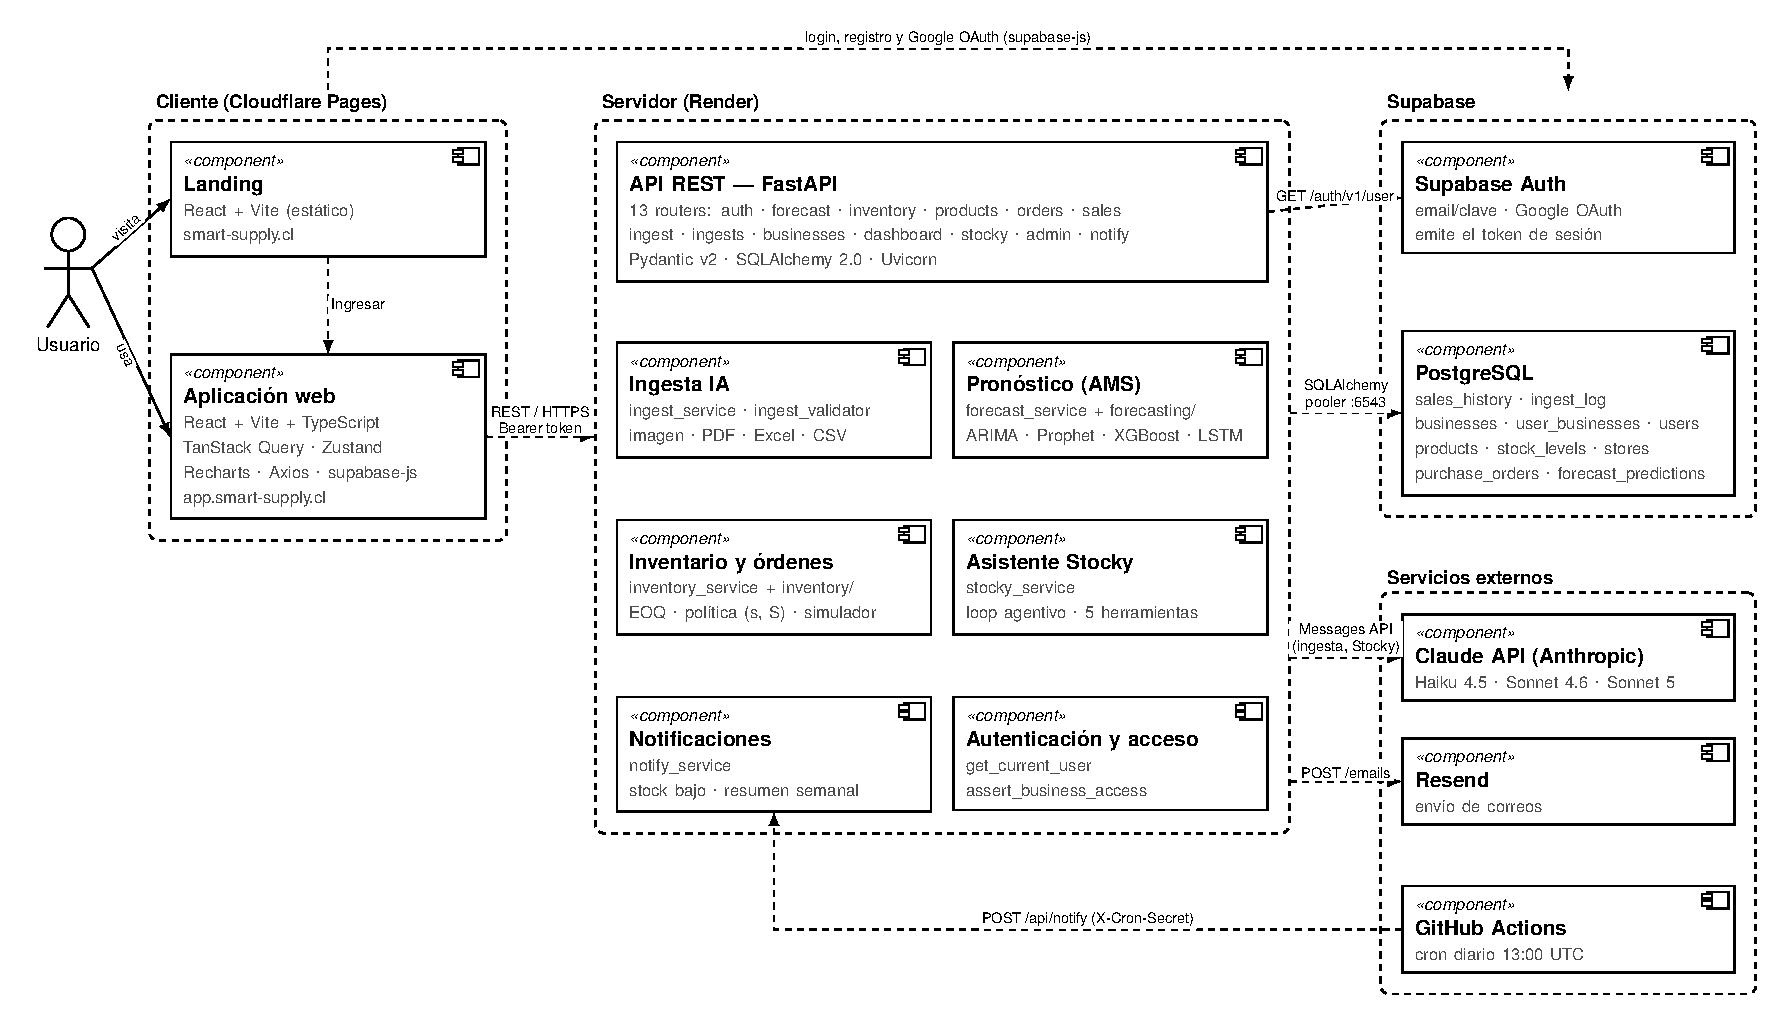
\includegraphics[angle=90, width=\textwidth, height=0.92\textheight, keepaspectratio]{figuras/componentes_uml.pdf}
  \caption{Diagrama de componentes de SmartSupply}
  \label{fig:componentes}
\end{figure}

La Tabla~\ref{tab:componentes-servidor} resume la responsabilidad de cada componente del
servidor y los archivos que lo implementan.

\begin{table}[H]
  \centering
  \caption{Componentes del servidor}
  \label{tab:componentes-servidor}
  \small
  \begin{tabular}{|p{2.6cm}|p{4.4cm}|p{6.6cm}|}
    \hline
    \textbf{Componente} & \textbf{Implementación} & \textbf{Responsabilidad} \\
    \hline
    API REST       & \texttt{app/main.py}, \texttt{app/api/}
                   & Expone los endpoints, valida las entradas con Pydantic y exige
                     autenticación en todas las rutas salvo las públicas. \\
    Ingesta IA     & \texttt{ingest\_service.py}, \texttt{ingest\_validator.py}
                   & Extrae registros de ventas, stock o productos desde imágenes, PDF,
                     Excel o CSV y revisa su calidad antes de cargarlos. \\
    Pronóstico     & \texttt{forecast\_service.py}, \texttt{forecasting/src/}
                   & Construye la serie de cada SKU y ejecuta el AMS para elegir el modelo
                     con menor error. \\
    Inventario     & \texttt{inventory\_service.py}, \texttt{inventory/src/}
                   & Calcula EOQ, la política $(s, S)$ y las alertas de stock, y genera
                     órdenes de compra. \\
    Stocky         & \texttt{stocky\_service.py}
                   & Asistente conversacional que consulta y actualiza productos, stock y
                     órdenes mediante herramientas. \\
    Notificaciones & \texttt{notify\_service.py}
                   & Envía por correo las alertas de stock bajo y el resumen semanal. \\
    Autenticación  & \texttt{app/api/auth.py}
                   & Valida el token de Supabase, crea la cuenta local en el primer ingreso
                     y verifica el acceso a cada negocio. \\
    \hline
  \end{tabular}
\end{table}

\section{Arquitectura de Despliegue}

El sistema se despliega por completo en plataformas gestionadas, lo que evita administrar
servidores y mantiene un costo fijo bajo durante el desarrollo
(Figura~\ref{fig:despliegue} y Tabla~\ref{tab:plataformas}).

\begin{figure}[p]
  \centering
  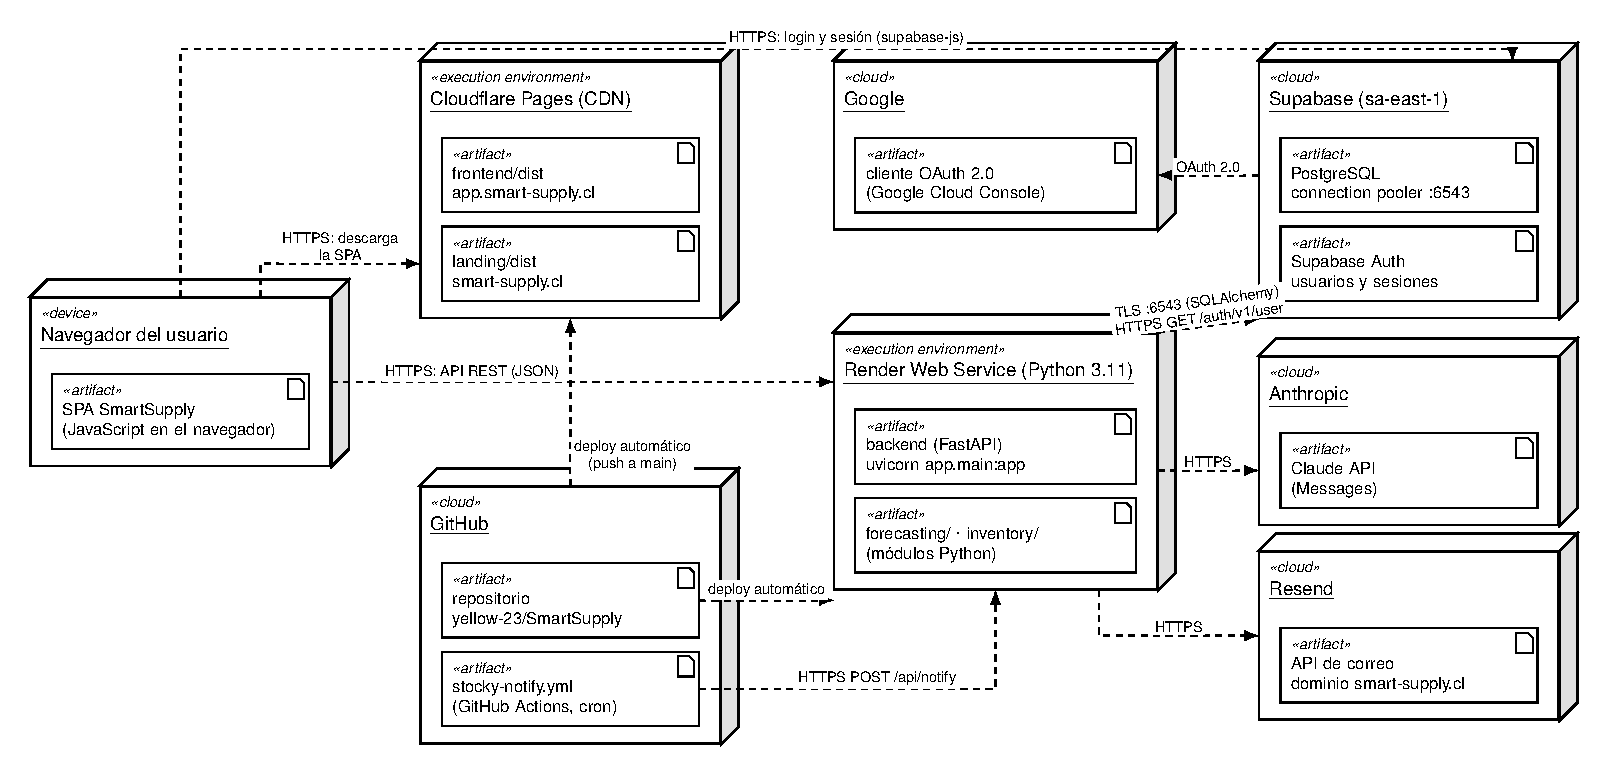
\includegraphics[angle=90, width=\textwidth, height=0.92\textheight, keepaspectratio]{figuras/despliegue_uml.pdf}
  \caption{Diagrama de despliegue de SmartSupply}
  \label{fig:despliegue}
\end{figure}

\begin{table}[H]
  \centering
  \caption{Plataformas de despliegue}
  \label{tab:plataformas}
  \small
  \begin{tabular}{|p{3.6cm}|p{4.2cm}|p{5.8cm}|}
    \hline
    \textbf{Elemento} & \textbf{Plataforma} & \textbf{Observaciones} \\
    \hline
    Aplicación web y landing & Cloudflare Pages
      & Sitios estáticos servidos desde CDN en \texttt{app.smart-supply.cl} y
        \texttt{smart-supply.cl}. \\
    API REST & Render (Web Service, plan Starter)
      & Python 3.11; el plan pagado evita que el servicio se suspenda por inactividad. \\
    Base de datos y autenticación & Supabase (región sa-east-1)
      & PostgreSQL con \textit{connection pooler} en el puerto 6543. El plan gratuito
        pausa el proyecto tras un periodo sin actividad. \\
    Modelos de lenguaje & Anthropic (Claude API) & Cobro por uso (tokens procesados). \\
    Correo electrónico & Resend & Envío desde el dominio \texttt{smart-supply.cl}. \\
    Código y tareas programadas & GitHub y GitHub Actions
      & Repositorio del proyecto y ejecución periódica de las notificaciones. \\
    \hline
  \end{tabular}
\end{table}

El despliegue es continuo: cada \textit{push} a la rama \texttt{main} dispara la
publicación automática del frontend en Cloudflare Pages y del backend en Render. La
configuración sensible se entrega mediante variables de entorno y nunca se guarda en el
repositorio: en Render, la cadena de conexión a la base de datos, la URL y la clave pública
de Supabase, la clave de la API de Anthropic, la clave de Resend y el secreto del cron; en
Cloudflare Pages, la URL de la API y los datos públicos de Supabase que el frontend
necesita al compilar.

\section{Modelo de Datos}

La base de datos tiene diez tablas (Figura~\ref{fig:base-datos}). Todas las tablas con
datos de un cliente incluyen \texttt{business\_id}, que actúa como clave de aislamiento
entre negocios según el modelo \textit{multi-tenant} descrito en el Marco Teórico. La
Tabla~\ref{tab:tablas} resume el propósito de cada una.

\begin{figure}[H]
  \centering
  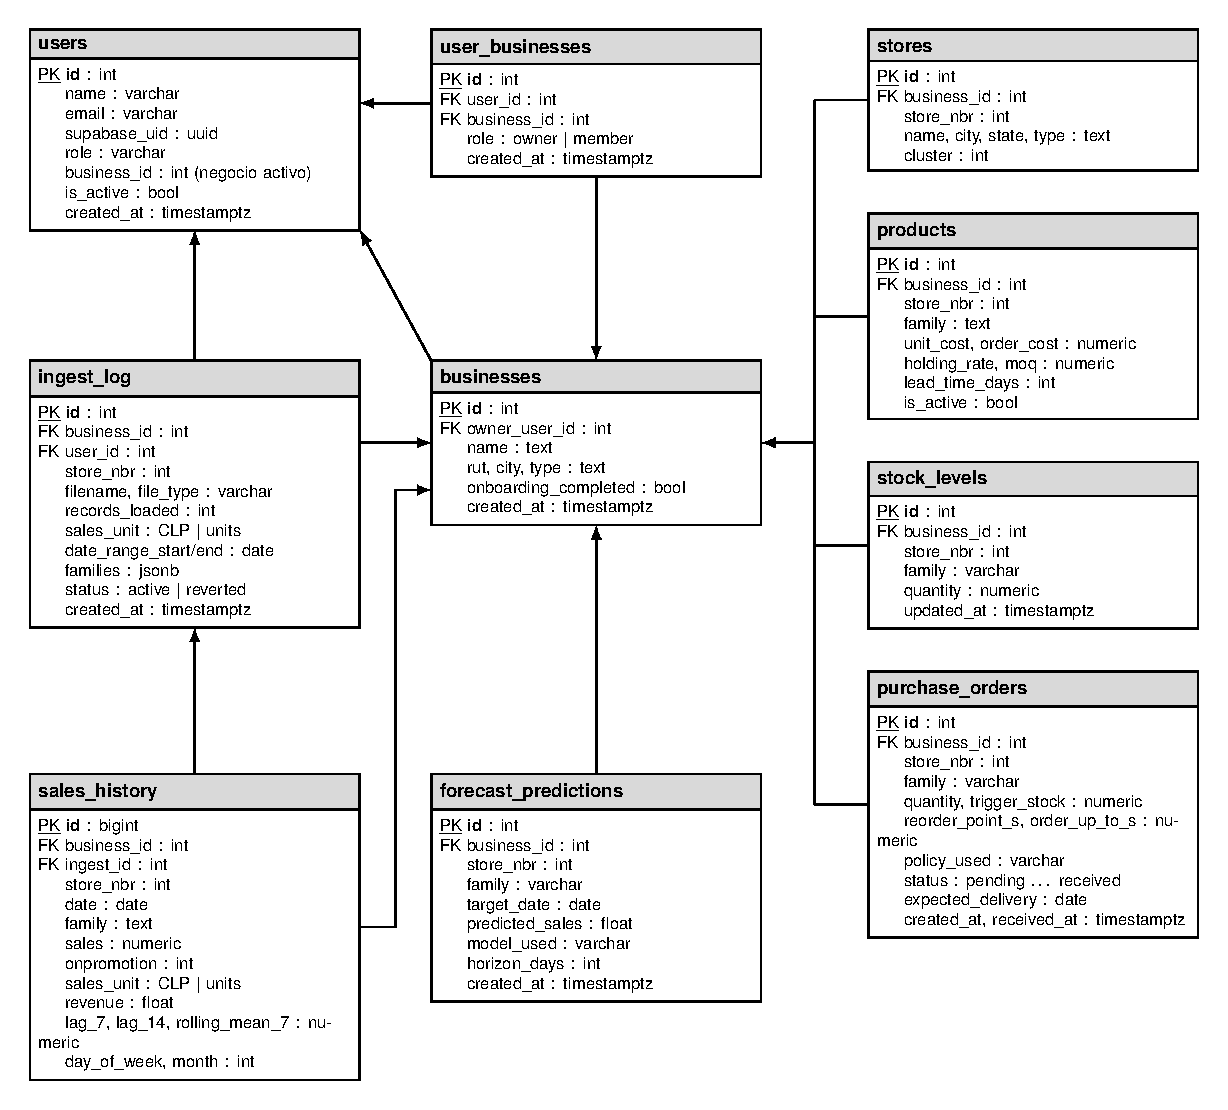
\includegraphics[width=\textwidth, height=0.8\textheight, keepaspectratio]{figuras/base_datos.pdf}
  \caption{Modelo de datos de SmartSupply (PostgreSQL)}
  \label{fig:base-datos}
\end{figure}

\begin{table}[H]
  \centering
  \caption{Tablas del modelo de datos}
  \label{tab:tablas}
  \small
  \begin{tabular}{|p{3.9cm}|p{9.7cm}|}
    \hline
    \textbf{Tabla} & \textbf{Propósito} \\
    \hline
    \texttt{users}                & Cuenta local de cada usuario, enlazada a Supabase Auth mediante
                                    \texttt{supabase\_uid}. El campo \texttt{role} identifica al
                                    administrador de la plataforma. \\
    \texttt{businesses}           & Negocios cliente de la plataforma; unidad de aislamiento de datos. \\
    \texttt{user\_businesses}     & Relación muchos a muchos entre usuarios y negocios, con rol
                                    \texttt{owner} o \texttt{member}. \\
    \texttt{stores}               & Sucursales o ubicaciones de cada negocio. \\
    \texttt{ingest\_log}          & Una fila por carga de datos: archivo, usuario, rango de fechas,
                                    familias incluidas y estado (\texttt{active} o \texttt{reverted}). \\
    \texttt{sales\_history}       & Ventas diarias por tienda y familia. Cada fila indica en
                                    \texttt{ingest\_id} la carga de la que proviene. \\
    \texttt{products}             & Parámetros de inventario por SKU: costo unitario, costo de pedido,
                                    tasa de mantención, \textit{lead time} y lote mínimo. Todos son
                                    opcionales. \\
    \texttt{stock\_levels}        & Stock actual por SKU y tienda. \\
    \texttt{purchase\_orders}     & Órdenes de compra generadas por la política $(s, S)$ y su estado. \\
    \texttt{forecast\_predictions} & Predicciones emitidas por el AMS, guardadas para compararlas con la
                                    venta real cuando esta se registre. \\
    \hline
  \end{tabular}
\end{table}

\subsection{Cargas versionadas}

Confirmar una carga no sobrescribe datos anteriores. Cada carga crea una fila en
\texttt{ingest\_log} e inserta sus propios registros en \texttt{sales\_history} con ese
\texttt{ingest\_id}; la restricción única \texttt{(business\_id, store\_nbr, date, family,
ingest\_id)} permite que dos cargas cubran el mismo día sin chocar.

Los solapamientos se resuelven al consultar, no al cargar: al construir una serie se
consideran solo las cargas con estado \texttt{active} y, si dos de ellas tienen un registro
para la misma fecha, se conserva el de la carga más reciente (mayor \texttt{ingest\_id}).
Revertir una carga solo cambia su estado a \texttt{reverted}: sus filas se conservan,
pero dejan de usarse en los cálculos. Eliminarla, en cambio, borra la carga y sus registros. Este diseño deja un historial
auditable de todo lo que se ha cargado y permite corregir errores sin perder información.

\section{Autenticación y Control de Acceso}

La identidad de los usuarios la gestiona Supabase Auth, que ofrece registro e ingreso con
correo y contraseña, ingreso con Google (OAuth 2.0) y recuperación de contraseña. El
frontend se comunica directamente con Supabase mediante la biblioteca
\texttt{supabase-js}, por lo que el backend nunca recibe ni almacena contraseñas.

Cada petición a la API incluye el token de sesión en la cabecera
\texttt{Authorization: Bearer}. La dependencia \texttt{get\_current\_user} lo valida
consultando \texttt{GET /auth/v1/user} en Supabase, en lugar de verificar la firma del
token localmente; así el backend no depende del esquema de firma que use el proyecto de
Supabase. La primera vez que aparece un usuario desconocido, el sistema crea
automáticamente su negocio, su tienda inicial y su cuenta local. Si ya existía una cuenta
con el mismo correo creada antes de la migración a Supabase Auth, se enlaza a la nueva
identidad sin perder sus datos. Como el ingreso con Google no permite pedir el nombre del
negocio, en ese caso se muestra una pantalla de configuración inicial antes de entrar a la
aplicación.

La autorización opera en dos niveles:

\begin{itemize}
  \item \textbf{Rol en la plataforma} (\texttt{users.role}): el rol \texttt{platform\_admin}
        habilita el panel de administración (\texttt{/admin}), desde donde se gestionan
        usuarios y negocios.
  \item \textbf{Rol en cada negocio} (\texttt{user\_businesses.role}): un \texttt{owner}
        tiene control total; un \texttt{member} puede consultar los datos, pero no revertir
        ni eliminar cargas.
\end{itemize}

Todo endpoint que recibe un \texttt{business\_id} verifica, mediante
\texttt{assert\_business\_access}, que el usuario pertenezca a ese negocio, y responde
\texttt{403} en caso contrario. Esta verificación impide que un usuario lea o modifique
datos de otro negocio cambiando un identificador en la petición. Como defensa adicional,
las políticas de Row Level Security de Supabase impiden leer las tablas con la clave
pública del proyecto. Los endpoints de notificaciones no los usa ningún usuario: los invoca
el cron y se protegen con un secreto compartido en la cabecera \texttt{X-Cron-Secret}.

\section{Ingesta de Datos Asistida por IA}

La ingesta es el mecanismo que permite a una distribuidora sin datos estructurados empezar
a usar el sistema. El usuario sube un archivo en el formato que tenga a mano (una foto de
un cuaderno, un PDF escaneado o una planilla con columnas propias) y el sistema lo
convierte en registros normalizados de fecha, familia y venta. El proceso tiene dos etapas,
vista previa y confirmación (Figura~\ref{fig:secuencia-ingesta}), para que ningún dato
llegue a la base sin que el usuario lo revise.

\begin{figure}[p]
  \centering
  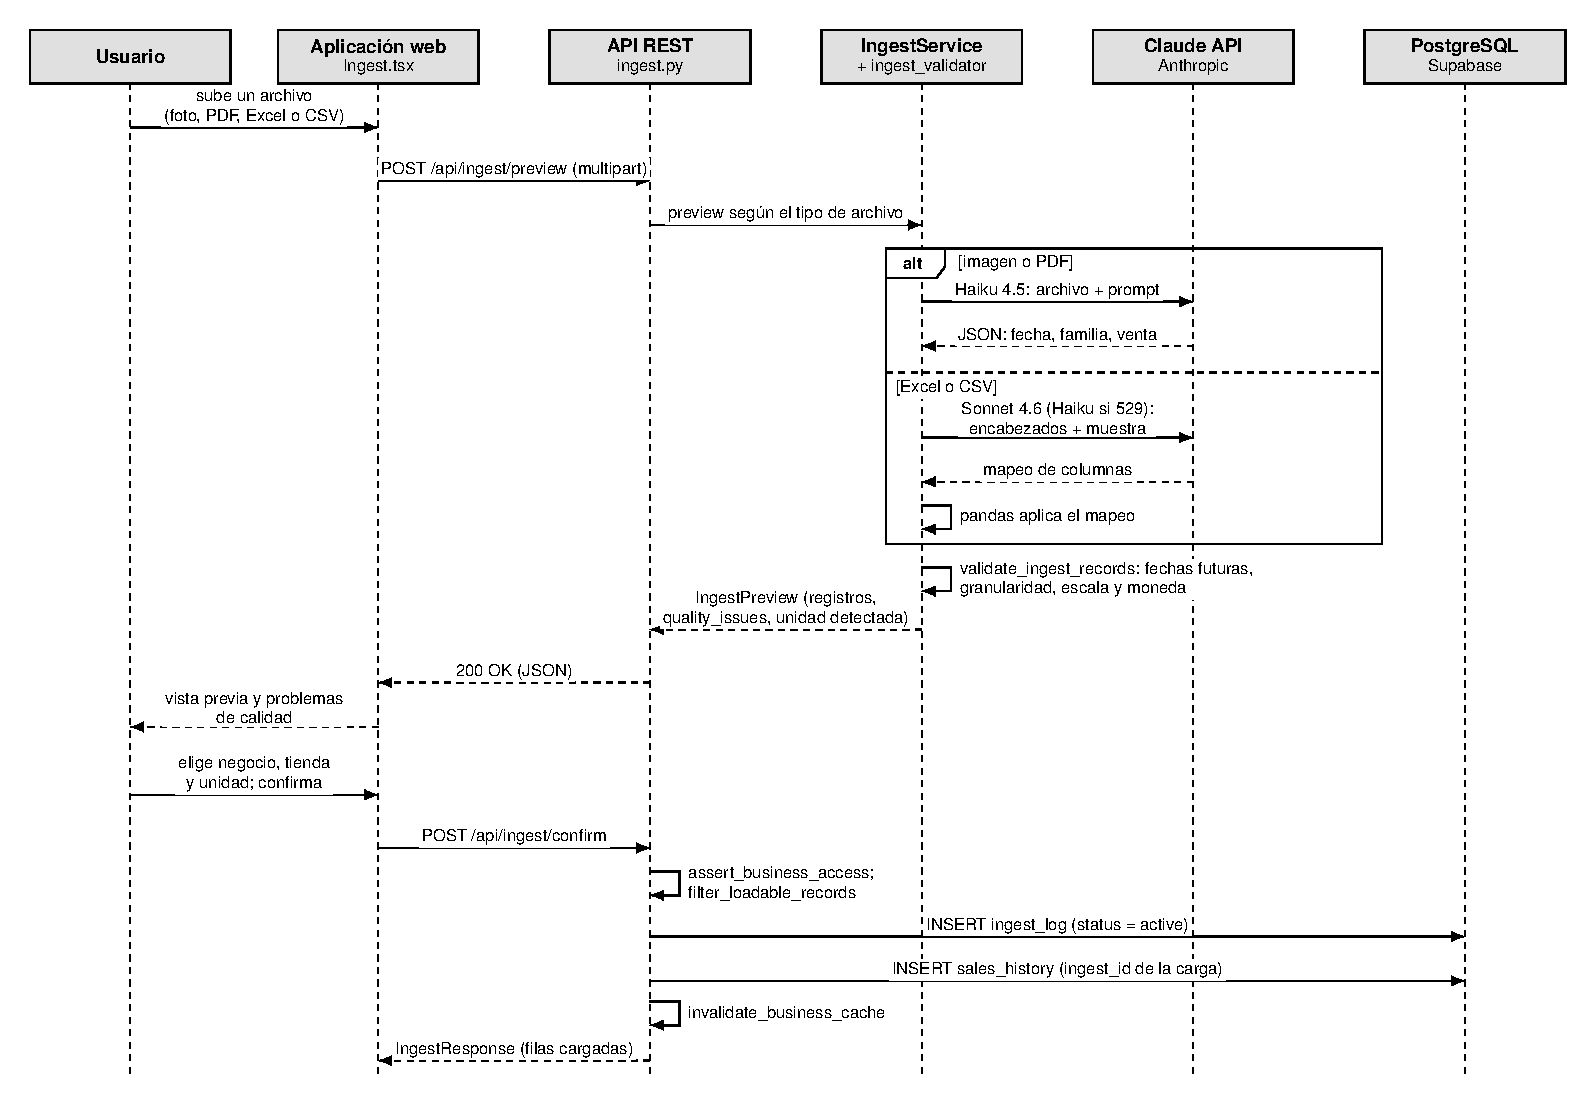
\includegraphics[angle=90, width=\textwidth, height=0.92\textheight, keepaspectratio]{figuras/secuencia_ingesta.pdf}
  \caption{Diagrama de secuencia de la ingesta asistida por IA}
  \label{fig:secuencia-ingesta}
\end{figure}

La estrategia de extracción depende del formato (Tabla~\ref{tab:ingesta-modelos}). En las
planillas, el modelo no procesa todas las filas: recibe los encabezados y una muestra y
devuelve qué columna corresponde a cada campo. Luego \texttt{pandas} aplica ese mapeo al
archivo completo, lo que reduce el costo en tokens y hace que la transformación de las
filas sea determinista.

\begin{table}[H]
  \centering
  \caption{Estrategia de extracción por formato de archivo}
  \label{tab:ingesta-modelos}
  \small
  \begin{tabular}{|p{2.8cm}|p{6.8cm}|p{4.0cm}|}
    \hline
    \textbf{Formato} & \textbf{Estrategia} & \textbf{Modelo} \\
    \hline
    Imagen (JPG, PNG, WEBP) & El modelo lee la imagen y devuelve los registros en JSON.
      & \texttt{claude-haiku-4-5} \\
    PDF & El modelo procesa el documento y devuelve los registros en JSON.
      & \texttt{claude-haiku-4-5} \\
    Excel o CSV & El modelo interpreta los encabezados y una muestra y devuelve el mapeo
      de columnas; \texttt{pandas} lo aplica a todas las filas.
      & \texttt{claude-sonnet-4-6}; si la API responde 529 (sobrecarga), \texttt{claude-haiku-4-5} \\
    \hline
  \end{tabular}
\end{table}

Antes de mostrar la vista previa, el validador de calidad revisa los registros extraídos y
reporta los problemas de la Tabla~\ref{tab:validador}. Los avisos se muestran con colores
según su severidad y se entregan también como contexto al asistente Stocky, que en la
pantalla de ingesta puede explicar al usuario qué significa cada uno y sugerir en qué
negocio y tienda cargar el archivo.

\begin{table}[H]
  \centering
  \caption{Controles del validador de calidad de la ingesta}
  \label{tab:validador}
  \small
  \begin{tabular}{|p{4.0cm}|p{2.2cm}|p{7.4cm}|}
    \hline
    \textbf{Código} & \textbf{Severidad} & \textbf{Condición} \\
    \hline
    \texttt{FUTURE\_DATES}        & Advertencia & Hay registros con fecha posterior a hoy. \\
    \texttt{MIXED\_GRANULARITY}   & Advertencia & Los intervalos entre fechas son inconsistentes:
                                                  el mayor supera 7 días y es más de 10 veces el menor
                                                  (por ejemplo, datos mensuales y diarios mezclados). \\
    \texttt{MONTHLY\_GRANULARITY} & Advertencia & El intervalo mediano entre fechas es de 25 días o más. \\
    \texttt{WEEKLY\_GRANULARITY}  & Información & El intervalo mediano está entre 5 y 25 días. \\
    \texttt{SCALE\_SHIFT}         & Advertencia & La mediana de ventas cambia más de 5 veces entre la
                                                  primera y la segunda mitad del periodo. \\
    \texttt{LIKELY\_CURRENCY}     & Advertencia & Al menos la mitad de las familias tiene una mediana
                                                  diaria sobre 10.000, lo que indica montos en pesos y no
                                                  unidades. \\
    \hline
  \end{tabular}
\end{table}

Al confirmar, el usuario elige el negocio y la tienda de destino e indica si las cifras son
unidades o montos en pesos (CLP). El backend verifica el acceso al negocio, descarta los
registros con fecha futura o venta cero, crea la carga en \texttt{ingest\_log}, inserta los
registros e invalida la caché de pronósticos del negocio. Además de ventas, el mismo flujo
acepta cargas de stock actual y de parámetros de productos.

\section{Pipeline de Pronóstico de Demanda}

El pronóstico de un SKU sigue la secuencia de la Figura~\ref{fig:secuencia-forecast}.

\begin{figure}[p]
  \centering
  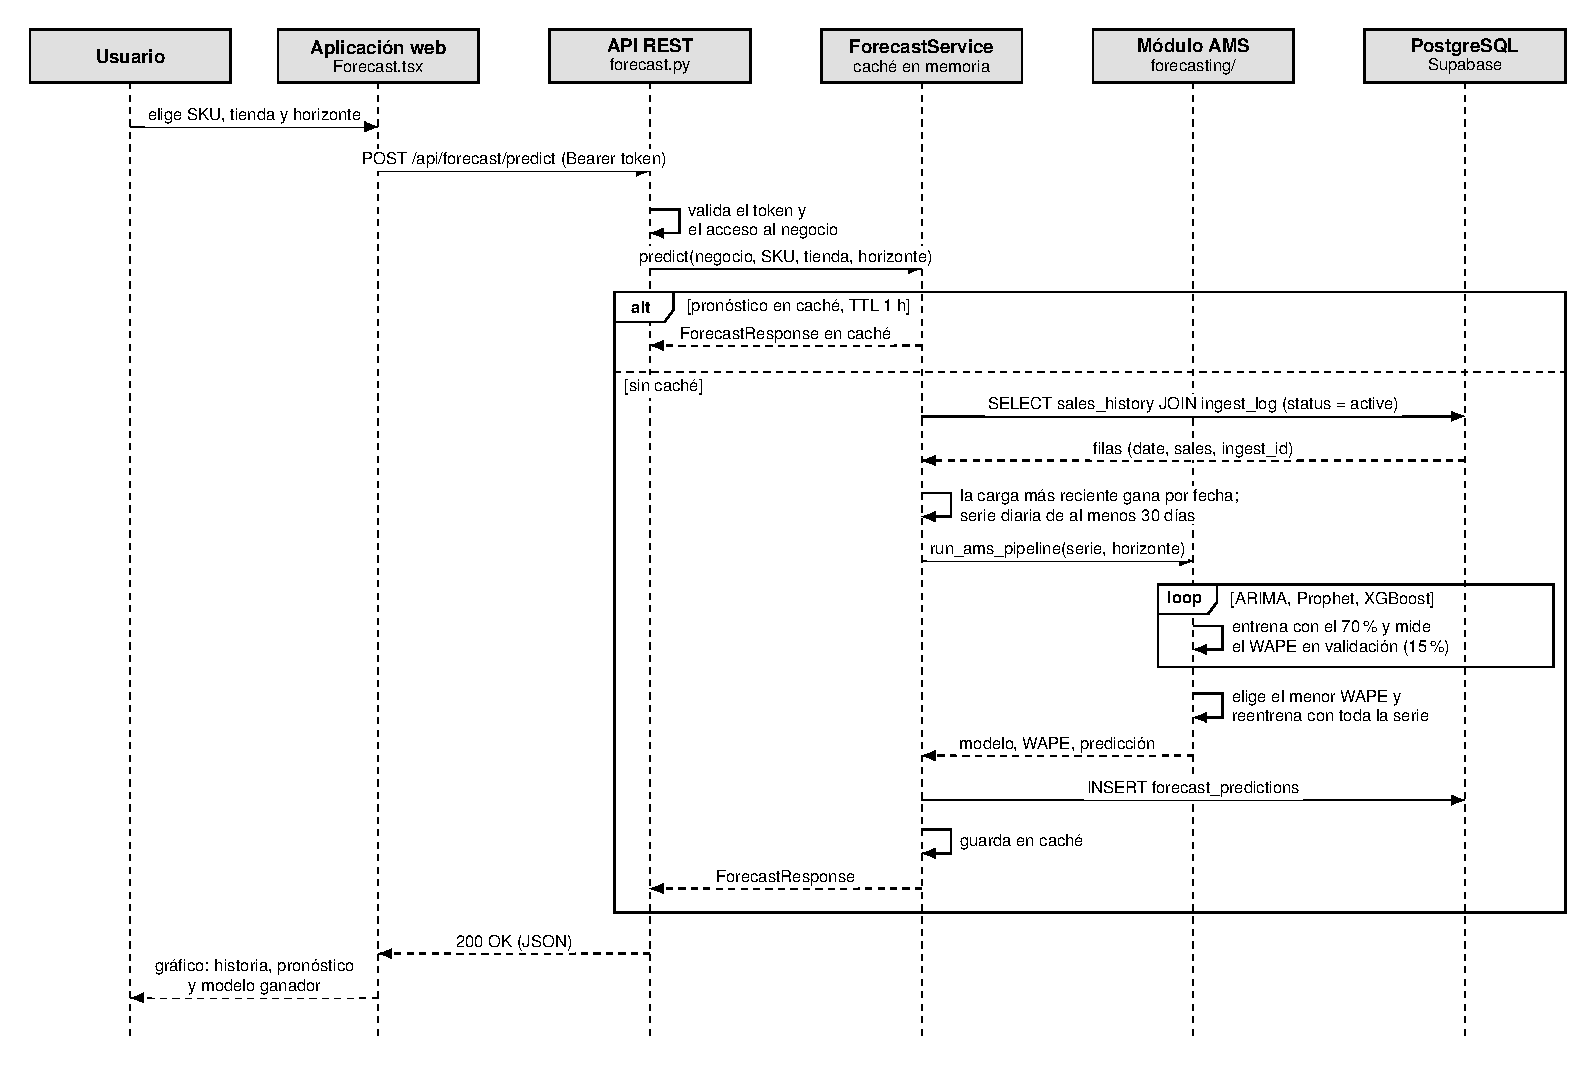
\includegraphics[angle=90, width=\textwidth, height=0.92\textheight, keepaspectratio]{figuras/secuencia_forecast.pdf}
  \caption{Diagrama de secuencia del pronóstico de demanda con AMS}
  \label{fig:secuencia-forecast}
\end{figure}

\begin{enumerate}
  \item \textbf{Construcción de la serie.} Se leen las ventas del SKU y la tienda desde las
        cargas activas, aplicando la regla de la carga más reciente. La serie se lleva a
        frecuencia diaria (los días sin registro quedan en cero), se excluyen las fechas
        futuras y se exigen al menos 30 días de historia.
  \item \textbf{Selección del modelo.} El AMS divide la serie en 70\,\% de entrenamiento,
        15\,\% de validación y 15\,\% de prueba. Cada modelo candidato se entrena con la
        primera parte y se mide su WAPE en validación. Se elige el de menor error, se
        reentrena con la serie completa y se proyecta el horizonte pedido (7, 14 o 30 días).
        En el modo automático de la API los candidatos son ARIMA, Prophet y XGBoost; LSTM
        está disponible cuando el usuario fuerza un modelo específico.
  \item \textbf{Caché.} El resultado se guarda en memoria durante una hora, con una clave
        que incluye negocio, SKU, tienda, horizonte y modelo. La caché del negocio se
        invalida cada vez que se carga, revierte, elimina o edita un dato de ventas, para no
        mostrar pronósticos basados en datos que ya cambiaron.
  \item \textbf{Registro para validación posterior.} Cada punto pronosticado se guarda en
        \texttt{forecast\_predictions}. Para cada fecha se conserva la primera predicción
        emitida, de modo que, cuando llega la venta real, el endpoint
        \texttt{GET /api/forecast/accuracy} calcula el error real del modelo con datos que
        no conocía al momento de predecir.
\end{enumerate}

\section{Inventario y Órdenes de Compra}

Para cada familia con ventas registradas, el servicio de inventario estima la demanda a
partir del historial y calcula el EOQ y los niveles de la política $(s, S)$ descritos en el
Marco Teórico. Los parámetros se toman de la tabla \texttt{products}; los que el usuario no
ha configurado usan valores por defecto: costo de pedido de 5.000, tasa de mantención de
0,25 y \textit{lead time} de 7 días.

El costo unitario no tiene un valor por defecto razonable: sin él, el EOQ entrega
cantidades desproporcionadas. Por eso, cuando falta, el SKU se marca como pendiente de
configuración y el sistema avisa en lugar de sugerir una cantidad. Si un SKU no tiene stock
registrado, se considera que su stock es cero; así, desde la primera carga todas las
familias aparecen en alerta hasta que el usuario ingresa su stock real.

Un SKU entra en alerta cuando su stock es menor o igual al punto de reorden $s$. La acción
\texttt{POST /api/orders/generate} crea una orden de compra por cada SKU en alerta que
tenga su costo configurado. Cada orden recorre los estados de la
Tabla~\ref{tab:estados-orden}; al marcarla como recibida, su cantidad se suma al stock de
la tienda.

\begin{table}[H]
  \centering
  \caption{Transiciones de estado de una orden de compra}
  \label{tab:estados-orden}
  \small
  \begin{tabular}{|l|l|}
    \hline
    \textbf{Estado actual} & \textbf{Estados siguientes permitidos} \\
    \hline
    \texttt{pending}    & \texttt{confirmed}, \texttt{cancelled} \\
    \texttt{confirmed}  & \texttt{in\_transit}, \texttt{cancelled} \\
    \texttt{in\_transit} & \texttt{received}, \texttt{cancelled} \\
    \texttt{received}   & (estado final) \\
    \texttt{cancelled}  & (estado final) \\
    \hline
  \end{tabular}
\end{table}

\section{Asistente Stocky}

Stocky es un asistente conversacional disponible como panel flotante en todas las páginas
de la aplicación. Funciona como un agente con herramientas: el modelo
(\texttt{claude-sonnet-5}) recibe la pregunta del usuario junto con la definición de cinco
herramientas sobre la base de datos (\texttt{list\_products}, \texttt{list\_stock\_levels},
\texttt{list\_orders}, \texttt{update\_product} y \texttt{update\_stock\_level}), decide
cuáles invocar y el backend las ejecuta dentro del negocio del usuario. El ciclo se repite
hasta que el modelo tiene una respuesta, con un máximo de seis iteraciones por mensaje.
Esto permite, por ejemplo, completar los costos de los productos o actualizar el stock
conversando, sin llenar formularios.

\section{Notificaciones Automáticas}

Un flujo de GitHub Actions invoca dos endpoints del backend a las 13:00 UTC (alrededor de
las 10:00 en Chile continental): todos los días \texttt{POST /api/notify/low-stock}, que
avisa al dueño de cada negocio qué productos están bajo su punto de reorden y cuánto pedir,
y los lunes \texttt{POST /api/notify/weekly-digest}, que resume las ventas de la última
semana con datos, el error promedio de los pronósticos, las órdenes pendientes y los
productos en alerta. Los correos se envían mediante la API de Resend. Ambos endpoints
aceptan un \texttt{business\_id} opcional, que se usa para probar los envíos con un único
negocio.

\section{API REST}

La API expone 55 endpoints agrupados en 13 \textit{routers} (Tabla~\ref{tab:routers}).
FastAPI genera a partir del código la documentación interactiva en formato OpenAPI,
disponible en la ruta \texttt{/docs} del backend.

\begin{table}[H]
  \centering
  \caption{Routers de la API REST}
  \label{tab:routers}
  \small
  \begin{tabular}{|l|p{10.4cm}|}
    \hline
    \textbf{Prefijo} & \textbf{Responsabilidad} \\
    \hline
    \texttt{/api/auth}       & Perfil del usuario autenticado, configuración inicial del negocio y un
                               ingreso de prueba para usar la documentación \texttt{/docs}. \\
    \texttt{/api/businesses} & Negocios del usuario y sus tiendas. \\
    \texttt{/api/ingest}     & Vista previa, confirmación y chat de la ingesta asistida por IA. \\
    \texttt{/api/ingests}    & Listado, detalle, reversión y eliminación de cargas. \\
    \texttt{/api/sales}      & Consulta del historial de ventas y edición de registros individuales. \\
    \texttt{/api/forecast}   & Pronóstico por SKU, precisión real, modelos disponibles y exportación a PDF. \\
    \texttt{/api/inventory}  & Alertas de stock, estado y métricas por SKU, y exportación a Excel. \\
    \texttt{/api/products}   & Mantención de los parámetros de inventario por SKU. \\
    \texttt{/api/orders}     & Órdenes de compra: generación, cambio de estado y exportación a Excel. \\
    \texttt{/api/dashboard}  & Indicadores y serie de ventas para la página de inicio. \\
    \texttt{/api/stocky}     & Chat con el asistente Stocky. \\
    \texttt{/api/admin}      & Gestión de usuarios y negocios (solo \texttt{platform\_admin}). \\
    \texttt{/api/notify}     & Disparo de las notificaciones por correo (solo el cron). \\
    \hline
  \end{tabular}
\end{table}

\end{document}
